\documentclass[a4paper, 12pt]{article}
\usepackage{deuresutils}
\usepackage{graphicx}
\usepackage{subcaption}
\usepackage{float}
\graphicspath{ {images/} }

\title{Pràctica 4}
\asignatura{Càlcul numèric}
\author{Eduardo Pérez Motato}
\niu{NIU: 1709992}
\date{30/05/2024}

\begin{document}
    \makeheader

    \begin{exercici}
        Considerar la interpolació polinòmica en la base de Newton amb diferències dividides per la funció
        $$
        f\left(x\right) = \frac{1}{1+25x^2};\; x\in \left[-1, 1\right]
        $$
        fent ús dos tipus de soport (nodes):
        \textbf{nodes equidistants} $x_j$
        $$
        x_j = -1 + j\frac{2}{n};\;j=0, \dots, n-1
        $$
        per $n = 4, 8, 16, 32, (64)$
        i \textbf{nodes de Txevitxov} $y_j$ definits com,
        $$
        y_j = \cos{\left(\frac{2j+1}{n+1}\frac{\pi}{2}\right)};\;j=0,\dots,n-1
        $$
        per $n = 4, 8, 16, 32, (64)$.
        \textbf{Atenció: el cas $n=64$ està al limit de presició i podrien sortir resultats poc
        consistents. Si aquest es el vostre cas, omitir el resultat i fer únicamnent $n = 4, 8, 16, 32.$}
        \begin{enumerate}[label=\alph*)]
            \item Calcular i dibuixar $f\left(x_k\right)$ i $p\left(x_k\right)$, en cadascun dels
            casos (nodes equidistants i de Txevitxov) pels valors $x_k = - 0.989 + 0.011k$, amb $k = 0, \dots, 180$
            (absises en $\left[-1, 1\right]$ que no coincideixen amb els nodes d'interpolació).\\
            \begin{solucio}
                Fet a \verb|Pr4Ex1a.c| i \verb|ploter.py|. El archiu de \verb|c| calcula les
                diferències dividides gràcies a una matriu de $n\times\left(n+1\right)$, amb la
                primera columna on està evaluat i a la segona el valor una vegada és evaluat. A partir
                d'alli contiuna omplent els valors de la matriu per la "diagonal" fins que té totes
                les diferències dividides. Després, a l'hora de evaluar amb la interpolació optinguda
                ho fa iterant per aquesta "columna". Després, desa tot a \verb|output.txt| i
                mitjançants el archiu de \verb|python| genera primer la grafica amb els nodes
                equidistants i després amb els de Txevitxov (ambdos comparats amb la funció original).\\
                Les grafiques generades són les seguents:
                \begin{figure}[H]
                    \begin{subfigure}{0.5\textwidth}
                        \centering
                        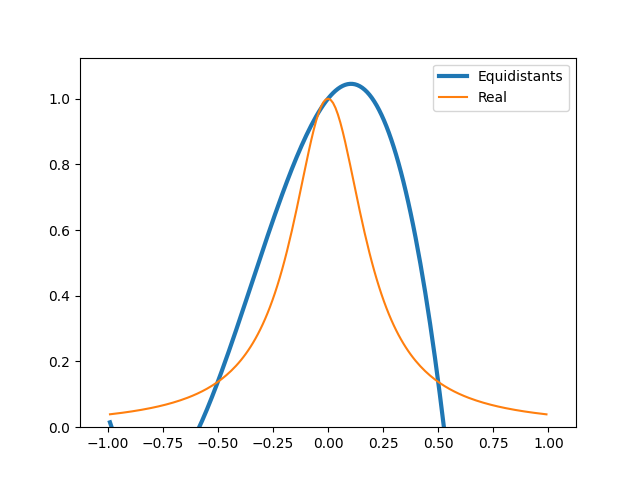
\includegraphics[width=\textwidth]{4_equi.png}
                        \caption{Equidistants}
                    \end{subfigure}
                    \begin{subfigure}{0.5\textwidth}
                        \centering
                        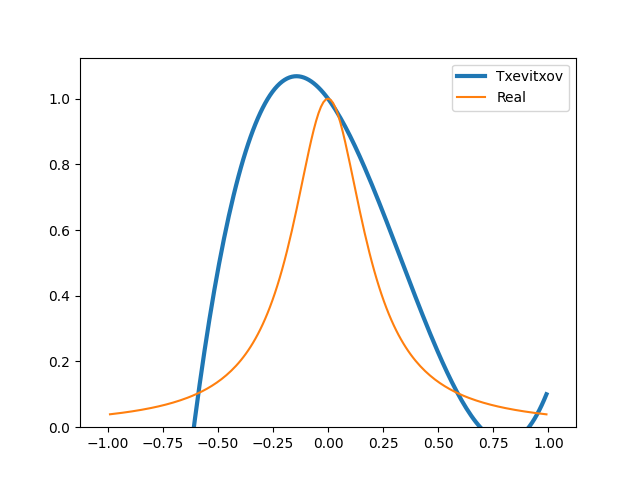
\includegraphics[width=\textwidth]{4_txev.png}
                        \caption{Txevitxov}
                    \end{subfigure}
                    \caption{4 nodes}
                \end{figure}
                \begin{figure}[H]
                    \begin{subfigure}{0.5\textwidth}
                        \centering
                        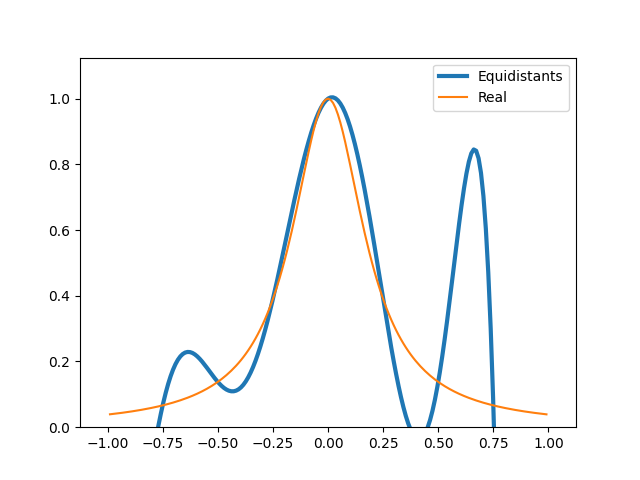
\includegraphics[width=\textwidth]{8_equi.png}
                        \caption{Equidistants}
                    \end{subfigure}
                    \begin{subfigure}{0.5\textwidth}
                        \centering
                        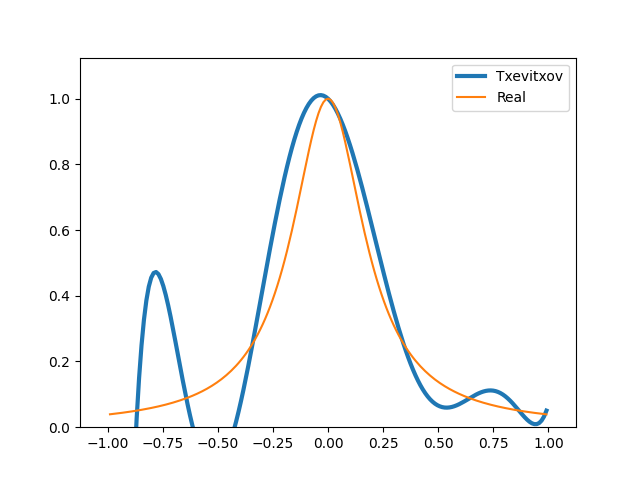
\includegraphics[width=\textwidth]{8_txev.png}
                        \caption{Txevitxov}
                    \end{subfigure}
                    \caption{8 nodes}
                \end{figure}
                \begin{figure}[H]
                    \begin{subfigure}{0.5\textwidth}
                        \centering
                        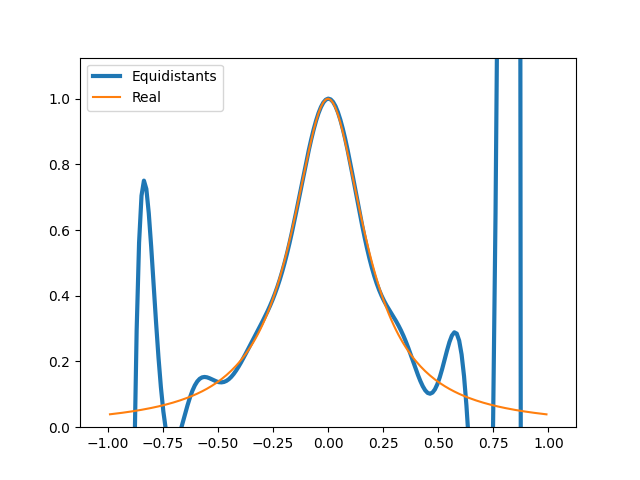
\includegraphics[width=\textwidth]{16_equi.png}
                        \caption{Equidistants}
                    \end{subfigure}
                    \begin{subfigure}{0.5\textwidth}
                        \centering
                        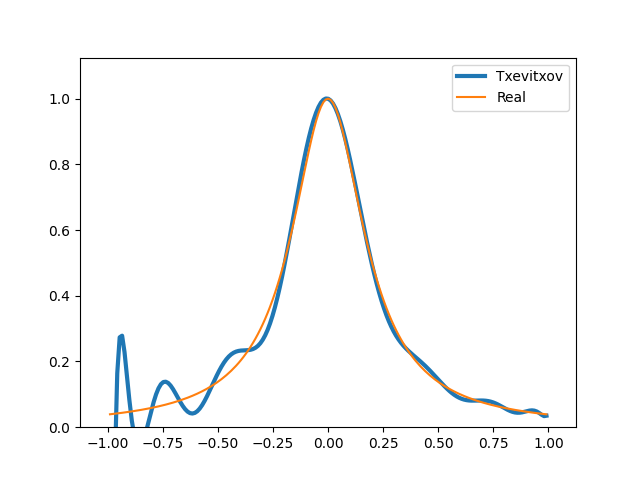
\includegraphics[width=\textwidth]{16_txev.png}
                        \caption{Txevitxov}
                    \end{subfigure}
                    \caption{16 nodes}
                \end{figure}
                \begin{figure}[H]
                    \begin{subfigure}{0.5\textwidth}
                        \centering
                        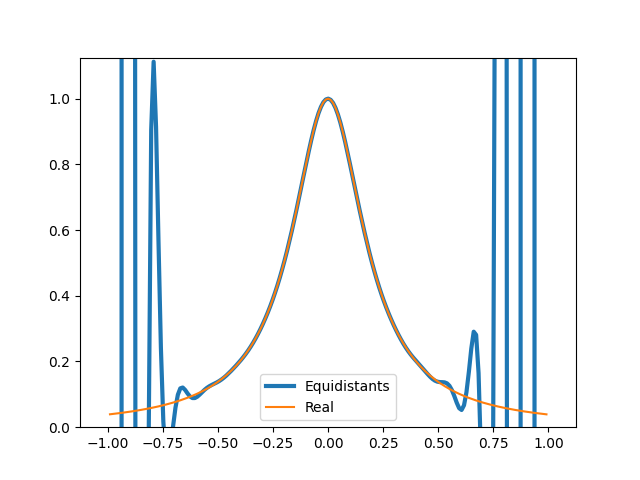
\includegraphics[width=\textwidth]{32_equi.png}
                        \caption{Equidistants}
                    \end{subfigure}
                    \begin{subfigure}{0.5\textwidth}
                        \centering
                        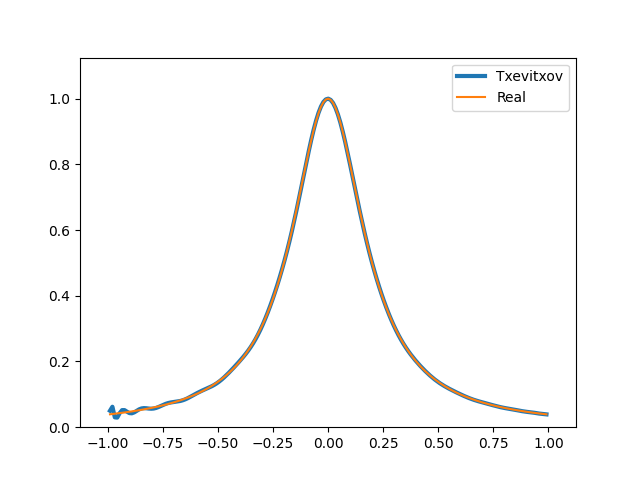
\includegraphics[width=\textwidth]{32_txev.png}
                        \caption{Txevitxov}
                    \end{subfigure}
                    \caption{32 nodes}
                \end{figure}
                Com es pot observar és poc simetrica. Aixó potser és per la manera de calcular els
                nodes (perquè hi hagui 16 nodes s'escullen del 0 al 15). Malgrat aixó, amb 32 nodes
                l'aproximació és molt bona. No he calculat amb 64 nodes perquè aixó provocaría més
                error pel límit de presició.
            \end{solucio}
            \item Comparar com es comporta l'error màxim que es comet a mesura que s'augmenta el
            nombre de nodes d'interpolació amb els diferents nodes d'interpolació i comentar els
            resultats (comparar $\left\lvert f\left(x_k\right)-p\left(x_k\right)\right\rvert$ i $\left\lvert f\left(y_k\right)-p\left(y_k\right)\right\rvert$
            per diferent nombre de nodes d'interpolació). \\
            \begin{solucio}
                A \verb|Pr4Ex1b.c| he fet un programa que calcula les diferències dividides (com a
                l'anterior apartat) però després demana punt al qual evaluarà aixó per trobar
                l'error i imprimir l'error d'ambdos per pantalla.\\
                A simple vista, amb 32 nodes l'error als extrems serà més alt pels equidistants. I
                si provem valors veiem que efectivament és cert. També podem observar que aixó
                passarà amb 16 nodes. Txevitxov no té aquest problema. Els errors són similars amb 8
                nodes, on a determinats llocs és millor equidistants.
            \end{solucio}
        \end{enumerate}
    \end{exercici}
\end{document}